
\subsection{Methodology}

All of our implementations were written in Java. Initially we thought of measuring the performance of our implementations with a naive approach where we would measure the time either in milliseconds or nanoseconds for sorting the input array. We could for example simply use \texttt{System.currentTimeMillis()} or \texttt{System.nanoTime()}. However we quickly found out how unreliable the results would be, since we noticed really inconsistent results between runs. As Ponge\cite{architectBenchmarking} explains, this kind of benchmarking might be viable in programs written in statically compiled languages like C. However Java runs on a Virtual Machine and it uses \emph{Just-in-time} compilation, so the first time the code is run it is actually being interpreted and then is compiled to native code, depending on the actual platform that is running. Furthermore, the VM tries to use all kinds of different optimization like loop unrolling, inlining functions or on-stack replacements, making it difficult to get consistent results. \\
We decided to use Java Microbenchmark Harness (JMH)\footnote{http://openjdk.java.net/projects/code-tools/jmh/} for measuring the performance of our implementations. JMH is an open source benchmarking tool part of the OpenJDK. Although it does not entirely prevent all common pitfalls and inconsistencies introduced by the JVM, it does help mitigating them. \\
Next step was to use the generated test cases files as inputs for our benchmarks. There are different modes to run benchmarks in JMH. We decided to measure the average time of an operation in microseconds, where an operation is sorting the array for any given algorithm and input array. In this mode, JMH considers an iteration to be a slice of time running as many operations as possible, it measures the time for each operation and averages it. In order to avoid some of the JIT inconsistencies and other JVM  optimizations, JMH runs a few warm-up iterations. After that it runs, by default, 5 iterations where the results are actually recorded. For our measuring purposes we decided to run 3  five seconds warm-up iterations and 5 ten seconds actual iterations.\\

The overall benchmark running time was over 36 hours. This was because we had large data sizes and due to the bad performance of some sorting algorithms in their worst case such as Bubble sort. We had to exclude Insertion and Bubble sort when running the test cases with a data size of 10,000,000.

\subsection{Results}
We ran the benchmark suite on a machine with an 4-cores and 8 logical processors @ 3.4Ghz and 24Gb of DDR4 RAM @ 3,401Mhz. The benchmark result reports can be found at \url{https://github.com/azeid/SortingAndSearchingAlgorithms/tree/master/results}. All the algorithms were run serially and nothing was parallelized. The benchmarks suite took around 36 hours where the majority of time was spent on Bubble and Insertion sorts since they were very slow. We ran data size of 10,000,000 for all the algorithms excluding Bubble and Insertions Sort; however, we did not include it since the results were linear with the data size and it was not adding any new information. We do have all the produces results and reports in our public GitHub repository \url{https://github.com/azeid/SortingAndSearchingAlgorithms}. In the graphs that we will use in this section the title of the graph will be the test case, they X-Axis is the data size and the Y-Axis is the time it took to sort the test case in microseconds.

\subsubsection{Interesting Observations}
In this section we will highlight some of the interesting observations that we found from our benchmark results since we cannot include all our graphs in the report due to space limitations; however, you can refer to the complete results and graphs in our public GitHub repository \url{https://github.com/azeid/SortingAndSearchingAlgorithms}. In Figure \ref{fig:allInDescendingOrder} we can see how bubble sort and insertion sort are very inefficient when it comes to sorting data compared to other sorting algorithms as the size of data increases, in fact we had to remove them from the final data comparison in order to see how the other algorithms performed compare to each other.

\begin{figure}[H]
\centering
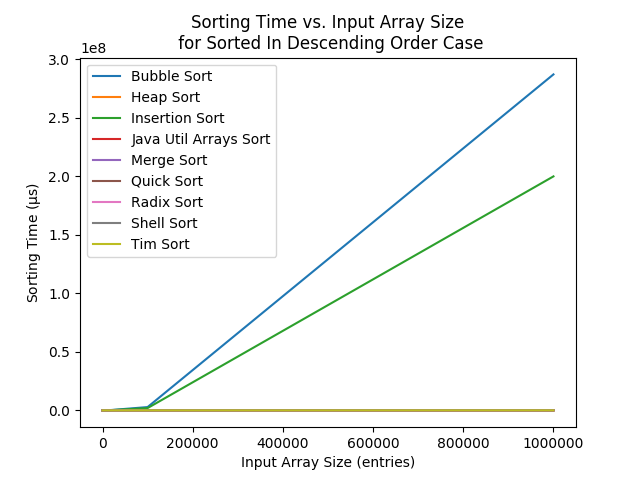
\includegraphics[width=9cm]{figures/plots_all_algs/sorting_time_vs_input_array_size_SortedInDescendingOrderCase.png}
\caption{All Algorithms - Data Sorted in Descending Order}
\label{fig:allInDescendingOrder}
\end{figure}

Another interesting observation is shown in Figure \ref{fig:allButBubbleInAscendingOrder} where the test case is of an array that is already sorted in ascending order i.e. best case. We can observe that insertion sort is as fast as the Java Utility Array Sort implementation, which is highly optimized, and see how other sorting algorithms still take some time even though the array is already sorted.

\begin{figure}[H]
\centering
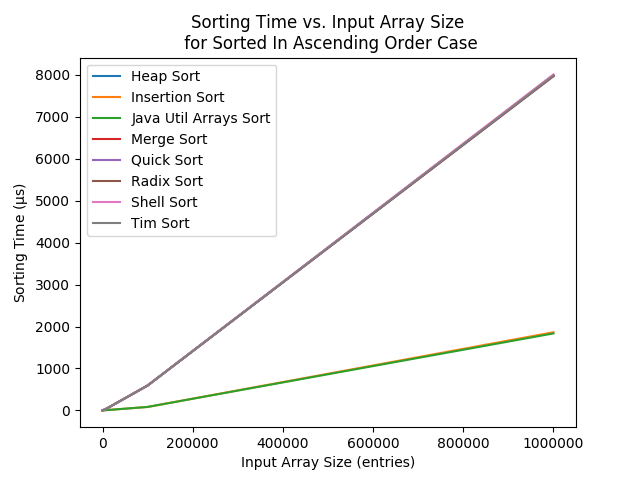
\includegraphics[width=9cm]{figures/plots_without_BubbleSort/sorting_time_vs_input_array_size_SortedInAscendingOrderCase.png}
\caption{All Algorithms Excluding Bubble Sort - Data Sorted in Ascending Order}
\label{fig:allButBubbleInAscendingOrder}
\end{figure}

\subsubsection{Final Results Excluding Bubble and Insertion Sort}

Below are the results for all the test cases for all sorting algorithms except Bubble Sort and Insertion Sort since they are too slow compared to other sorting algorithms and would hide the relative differences between the other algorithms if included.

\begin{figure}[!htp]
\centering
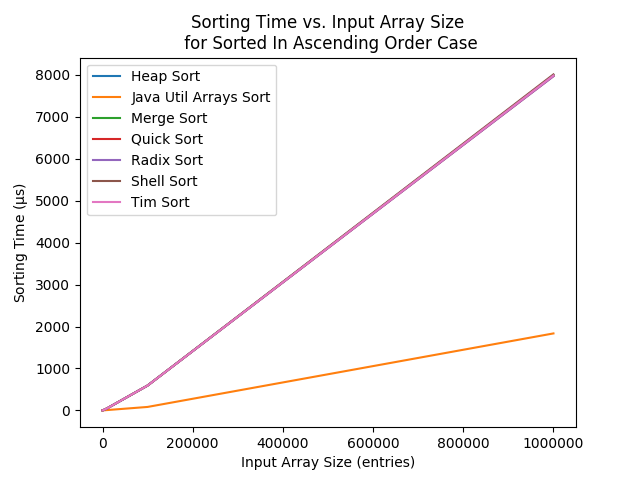
\includegraphics[width=9cm]{figures/plots_without_BubbleSort_InsertionSort/sorting_time_vs_input_array_size_SortedInAscendingOrderCase.png}
\end{figure}

\begin{figure}[!htp]
\centering
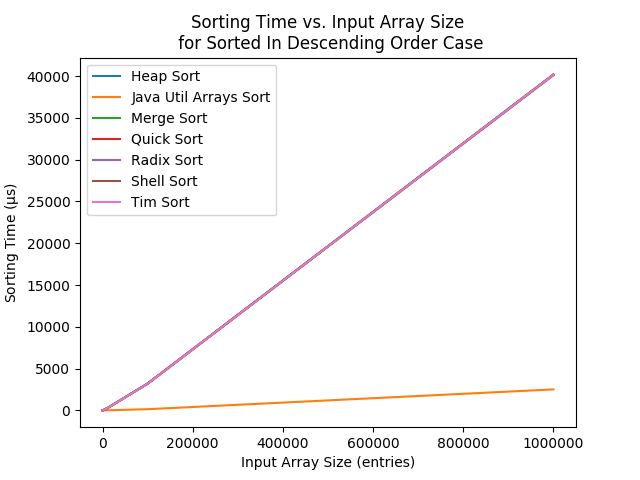
\includegraphics[width=9cm]{figures/plots_without_BubbleSort_InsertionSort/sorting_time_vs_input_array_size_SortedInDescendingOrderCase.png}
\end{figure}

\begin{figure}[!htp]
\centering
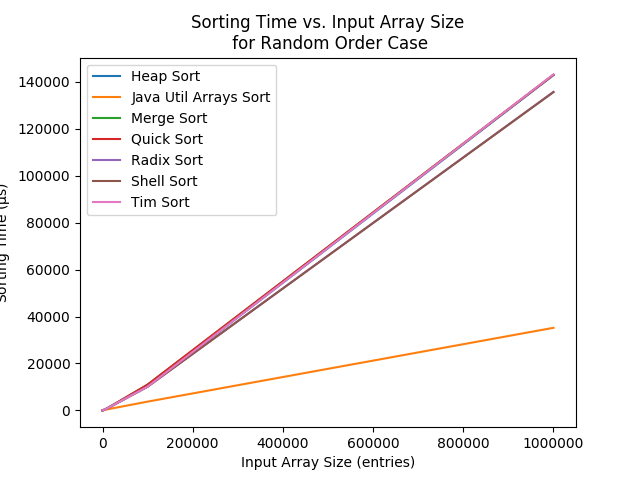
\includegraphics[width=9cm]{figures/plots_without_BubbleSort_InsertionSort/sorting_time_vs_input_array_size_RandomOrderCase.png}
\end{figure}

\begin{figure}[!htp]
\centering
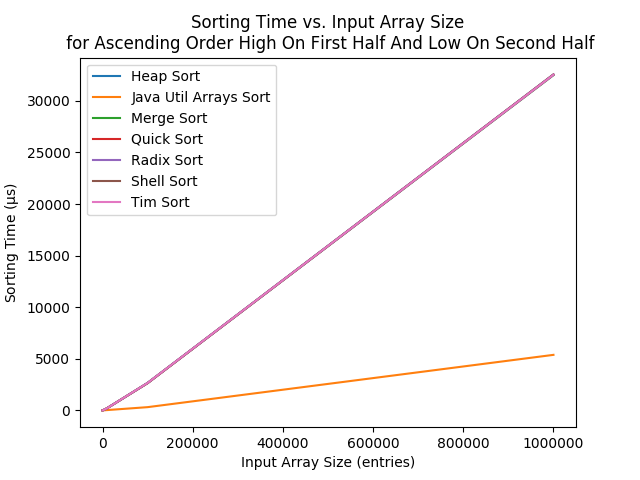
\includegraphics[width=9cm]{figures/plots_without_BubbleSort_InsertionSort/sorting_time_vs_input_array_size_AscendingOrderHighOnFirstHalfAndLowOnSecondHalf.png}
\end{figure}

\begin{figure}[!htp]
\centering
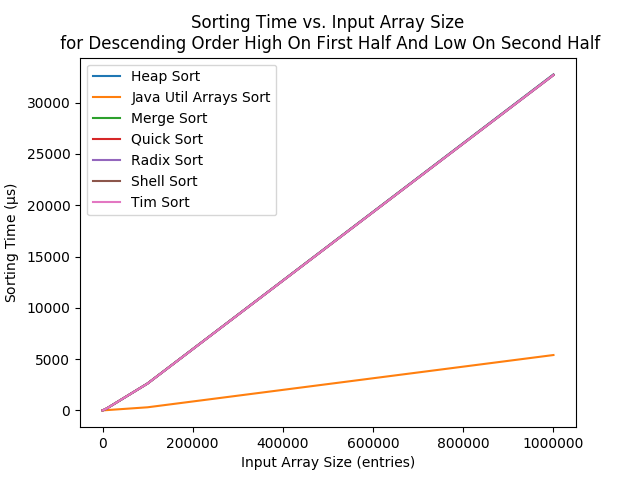
\includegraphics[width=9cm]{figures/plots_without_BubbleSort_InsertionSort/sorting_time_vs_input_array_size_DescendingOrderHighOnFirstHalfAndLowOnSecondHalf.png}
\end{figure}

\begin{figure}[!htp]
\centering
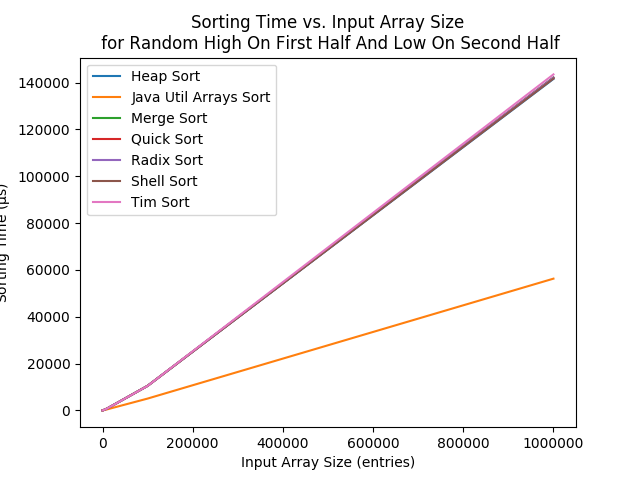
\includegraphics[width=9cm]{figures/plots_without_BubbleSort_InsertionSort/sorting_time_vs_input_array_size_RandomHighOnFirstHalfAndLowOnSecondHalf.png}
\end{figure}

\begin{figure}[!htp]
\centering
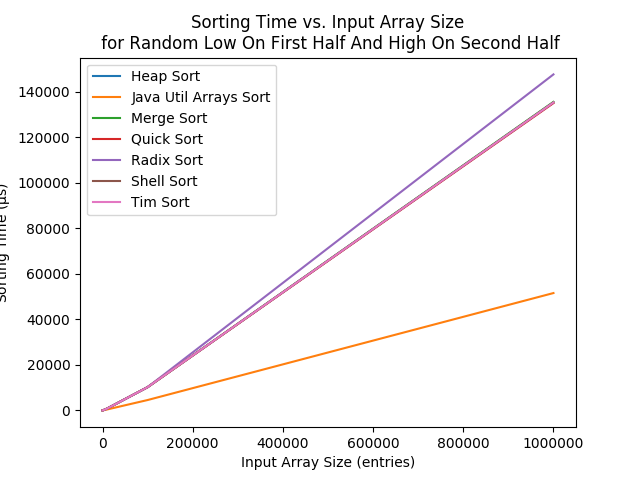
\includegraphics[width=9cm]{figures/plots_without_BubbleSort_InsertionSort/sorting_time_vs_input_array_size_RandomLowOnFirstHalfAndHighOnSecondHalf.png}
\end{figure}

\begin{figure}[!htp]
\centering
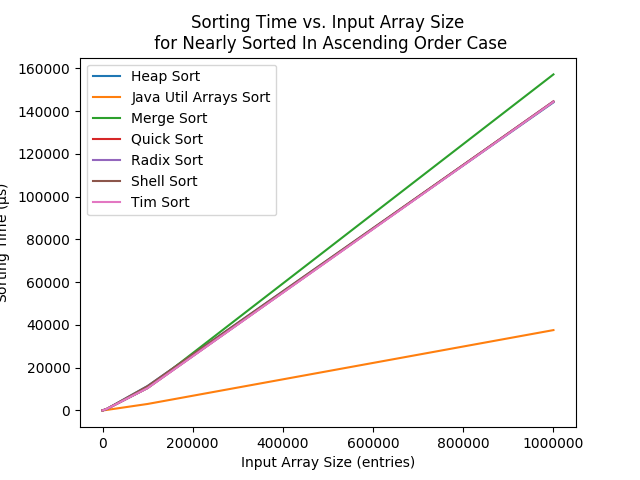
\includegraphics[width=9cm]{figures/plots_without_BubbleSort_InsertionSort/sorting_time_vs_input_array_size_NearlySortedInAscendingOrderCase.png}
\end{figure}

\begin{figure}[!htp]
\centering
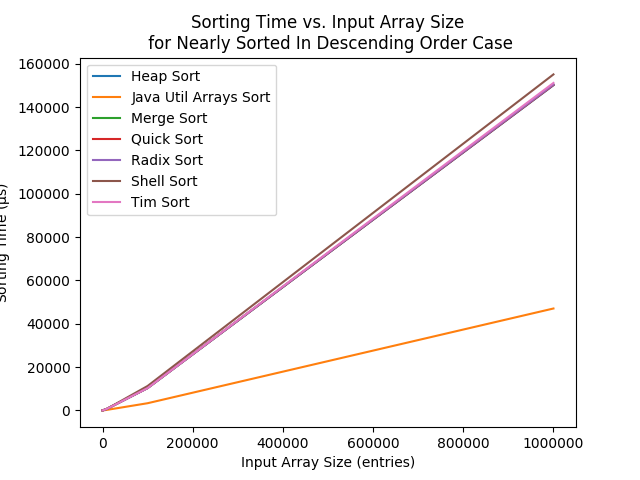
\includegraphics[width=9cm]{figures/plots_without_BubbleSort_InsertionSort/sorting_time_vs_input_array_size_NearlySortedInDescendingOrderCase.png}
\end{figure}

\begin{figure}[!htp]
\centering
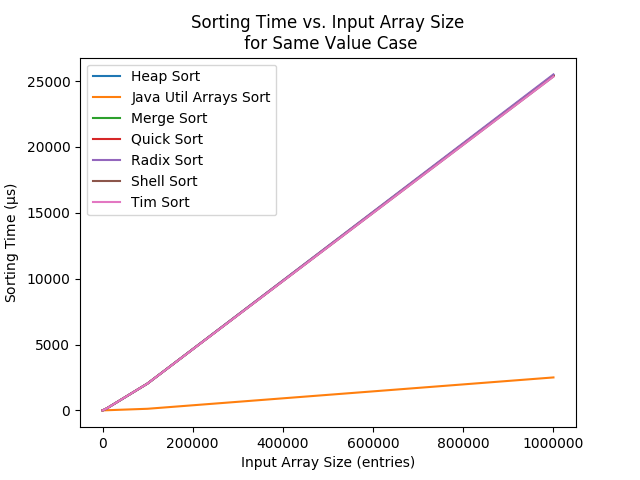
\includegraphics[width=9cm]{figures/plots_without_BubbleSort_InsertionSort/sorting_time_vs_input_array_size_SameValueCase.png}
\end{figure}

\begin{figure}[!htp]
\centering
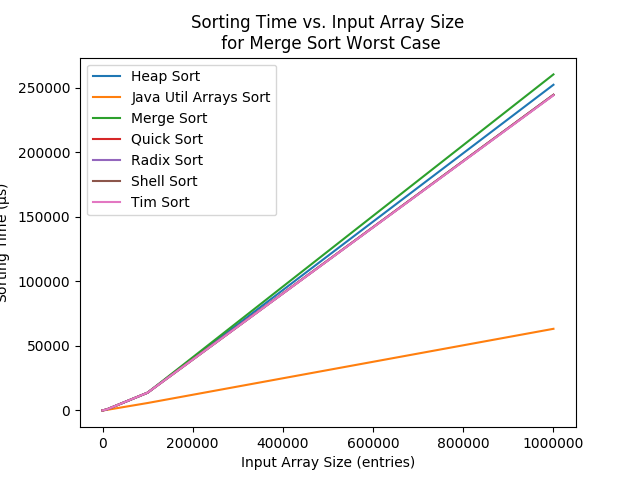
\includegraphics[width=9cm]{figures/plots_without_BubbleSort_InsertionSort/sorting_time_vs_input_array_size_MergeSortWorstCase.png}
\end{figure}